\subsection{\texorpdfstring{\(\mathfrak{S}\)-CONVERGENCE IN SPACES OF CONTINUOUS MAPPINGS}{S-CONVERGENCE IN SPACES OF CONTINUOUS MAPPINGS}}

Let X, Y be two topological spaces, and let C(X; Y) denote the set of all continuous mappings of X into Y. If S is a set of subsets of X and if Y is a uniform space, we denote by \(\mathcal{C}_{\mathfrak{S}}(\mathbf{X};\mathbf{Y})\) the set C(X; Y) endowed with the uniformity of S-convergence. In particular \(\mathcal{C}_{s}(\mathbf{X};\mathbf{Y})\) , \(\mathcal{C}_{c}(\mathbf{X};\mathbf{Y})\) and \(\mathcal{C}_{u}(\mathbf{X};\mathbf{Y})\) denote the set C(X; Y) endowed respectively with the uniformity of pointwise convergence, compact convergence and uniform convergence.

PROPOSITION 6. Let X be a topological space, Y a uniform space and S a set of subsets of X. For each A ∈ S and each closed entourage V of Y, the traces on C (X; Y) × C (X; Y) of W(A, V) and W(A̅, V) are the same.

For if \(u, v\) are continuous mappings of \(\mathbf{X}\) into \(\mathbf{Y}\) , the mapping \(x \to (u(x), v(x))\) of \(\mathbf{X}\) into \(\mathbf{Y} \times \mathbf{Y}\) is continuous, and the hypothesis that \((u(x), v(x)) \in \mathbf{V}\) for all \(x \in \mathbf{A}\) therefore implies that \((u(x), v(x)) \in \overline{\mathbf{V}} = \mathbf{V}\) for all \(x \in \overline{\mathbf{A}}\) (Chapter I, § 2, no. 1, Theorem 1).

If \(\overline{\mathfrak{S}}\) denotes the set of closures in \(\mathbf{X}\) of the sets of \(\mathfrak{S}\) , Proposition 6 shows that, on \(\mathcal{C}(\mathbf{X};\mathbf{Y})\) , the structures of \(\mathfrak{S}\) -convergence and \(\overline{\mathfrak{S}}\) -convergence are identical.

COROLLARY. Let B be a dense subset of X. On C(X; Y), the structure of uniform convergence is identical with the structure of uniform convergence in B.

PROPOSITION 7. Let X be a topological space, let S be a set of subsets of X and let Y be a uniform space. If Y is Hausdorff and if the union B of the sets of S is dense in X, then \(\mathcal{C}_{\mathfrak{S}}(X;Y)\) is Hausdorff.

For if \((u, v)\) belongs to all the sets \(W(A, V)\) , where \(A \in \mathfrak{S}\) and \(V\) is an entourage of \(Y\) , the hypothesis that \(Y\) is Hausdorff tells us that \(u(x) = v(x)\) for all \(x \in B\) ; if \(u\) and \(v\) are continuous, then \(u = v\) by the principle of extension of identities (Chapter I, §8, no. 1, Proposition 2, Corollary 1).

In particular, on \(\mathcal{C}(\mathbf{X};\mathbf{Y})\) , the topology of pointwise convergence in a dense subset of \(\mathbf{X}\) is Hausdorff.

PROPOSITION 8. Let X be a set, F a filter on X, and let Y be a uniform space. Then the set H of mappings \(u: \mathbf{X} \to \mathbf{Y}\) such that \(u(\mathfrak{F})\) is a Cauchy filter base on Y is closed in \(\mathcal{F}_u(\mathbf{X}; \mathbf{Y})\) .

Let \(u_0: \mathbf{X} \to \mathbf{Y}\) lie in the closure of \(\mathbf{H}\) in \(\mathcal{F}_u(\mathbf{X}; \mathbf{Y})\) . For each symmetric entourage \(\mathbf{V}\) of \(\mathbf{Y}\) , there is a mapping \(u \in \mathbf{H}\) such that \((u_0(x), u(x)) \in \mathbf{V}\) for all \(x \in \mathbf{X}\) ; on the other hand, by hypothesis there is a set \(\mathbf{M} \in \mathfrak{F}\) such that \((u(x), u(x')) \in \mathbf{V}\) whenever \(x\) and \(x'\) are in \(\mathbf{M}\) . Since \((u_0(x), u(x)) \in \mathbf{V}\) and \((u_0(x'), u(x')) \in \mathbf{V}\) , it follows that \((u_0(x), u_0(x')) \in \overset{3}{\mathbf{V}}\) whenever \(x\) and \(x'\) are in \(\mathbf{M}\) , and therefore \(u_0(\mathfrak{F})\) is a Cauchy filter base on \(\mathbf{Y}\) .

COROLLARY I. Let X be a topological space and Y a uniform space. The set of mappings of X into Y which are continuous at a point \(x_{0} \in X\) is closed in \(\mathcal{F}_{u}(X; U)\) .

If V is the neighbourhood filter of \(x_{0}\) in X, \(u(x_{0})\) is a cluster point of \(u(\mathbf{V})\) ; hence u is continuous at \(x_{0}\) if and only if \(u(\mathbf{V})\) is a Cauchy filter base on Y (Chapter II, §3, no. 2, Proposition 5, Corollary 2).

COROLLARY 2. Let X, L be two sets filtered by filters F, G respectively, and let Y be a complete uniform space. For each \(\lambda \in L\) , let \(u_{\lambda}\) be a mapping of X into Y. Suppose that (i) the family \((u_{\lambda})_{\lambda \in L}\) converges uniformly in X (with respect to the filter G) to a mapping \(v: X \to Y\) ; (ii) for each \(\lambda \in L\) , \(u_{\lambda}\) has a limit \(y_{\lambda}\) with respect to the filter F. Under these conditions, \(v\) has a limit with respect to F, and every limit of \(v\) with respect to F is a limit of the family \((y_{\lambda})_{\lambda \in L}\) with respect to G.

For \(v\) lies in the closure of the set of the \(u_{\lambda}\) in \(\mathcal{F}_u(\mathbf{X};\mathbf{Y})\) , and therefore \(v(\mathfrak{F})\) is a Cauchy filter base on \(\mathbf{Y}\) by virtue of Proposition 8; this shows that \(v\) has a limit \(y\) with respect to \(\mathfrak{F}\) because \(\mathbf{Y}\) is complete. Let

\(X' = X \cup \{\omega\}\) be the topological space associated with the filter \(\mathfrak{F}\) (Chapter I, § 6, no. 5), and extend \(u_{\lambda}\) (resp. \(v\) ) to a mapping \(\overline{u}_{\lambda}\) (resp. \(\overline{v}\) ) of \(X'\) into Y by putting \(\overline{u}_{\lambda}(\omega) = y_{\lambda}\) {[}resp. \(\overline{v}(\omega) = y\) {]}. Then the mappings \(\overline{u}_{\lambda}, \overline{v}\) are continuous on \(X'\) , and \(\overline{u}_{\lambda}\) converges uniformly in X to \(\overline{v}\) with respect to \(\mathfrak{G}\) ; since X is dense in \(X'\) , the Corollary to Proposition 6 shows that \(\overline{u}_{\lambda}\) converges uniformly in \(X'\) to \(\overline{v}\) , and in particular that \(y = \lim_{\mathfrak{G}} y_{\lambda}\) .

THEOREM 2. Let X be a topological space, Y a uniform space. Then the set C(X; Y) of continuous mappings of X into Y is a closed subset of the space F(X; Y) endowed with the topology of uniform convergence.

For each \(x \in \mathbf{X}\) , the set of mappings of \(\mathbf{X}\) into \(\mathbf{Y}\) which are continuous at \(x\) is closed in \(\mathcal{F}_u(\mathbf{X};\mathbf{Y})\) (Proposition 8, Corollary 1); hence the intersection \(\mathcal{C}(\mathbf{X};\mathbf{Y})\) of these sets is also closed.

This result may be expressed in the form that the uniform limit of continuous functions is continuous.

COROLLARY I. If Y is a complete uniform space, then \(\mathcal{C}_{u}(\mathbf{X};\mathbf{Y})\) is complete. For, by Theorem 2, \(\mathcal{C}_{u}(\mathbf{X};\mathbf{Y})\) is a closed uniform subspace of the uniform space \(\mathcal{F}_{u}(\mathbf{X};\mathbf{Y})\) , which is complete by Theorem 1 of no. 5.

COROLLARY 2. Let X be a topological space, S a set of subsets of X, and Y a uniform space. Let \(\tilde{\mathcal{C}}_{\mathfrak{S}}(X;Y)\) denote the set of all mappings of X into Y whose restriction to each set of S is continuous. Then \(\tilde{\mathcal{C}}_{\mathfrak{S}}(X;Y)\) is a closed subspace of the uniform space \(\mathcal{F}_{\mathfrak{S}}(X;Y)\) and is complete if Y is complete.

Suppose that \(u\) lies in the closure of \(\tilde{\mathcal{C}}_{\mathfrak{S}}(\mathbf{X};\mathbf{Y})\) in \(\mathcal{F}_{\mathfrak{S}}(\mathbf{X};\mathbf{Y})\) ; then (no. 2), for each \(\mathbf{A} \in \mathfrak{S}\) , \(u|\mathbf{A}\) lies in the closure of \(\mathcal{C}(\mathbf{A};\mathbf{Y})\) in \(\mathcal{F}_u(\mathbf{A};\mathbf{Y})\) , and is therefore continuous by Theorem 2.

COROLLARY 3. Let X be a topological space which is either metrizable or locally compact, and let Y be a uniform space. Then \(\mathcal{C}(\mathbf{X};\mathbf{Y})\) is closed in the uniform space \(\mathcal{F}_c(\mathbf{X};\mathbf{Y})\) ; if in addition Y is complete, the uniform space \(\mathcal{C}_c(\mathbf{X};\mathbf{Y})\) is complete.

By virtue of Corollary 2 it is enough to show that, if we take \(\mathfrak{S}\) to be the set of compact subsets of X, we have \(\tilde{\mathcal{C}}_{\mathfrak{S}}(X;Y) = \mathcal{C}(X;Y)\) in both cases under consideration. This is clear if X is locally compact. If X is metrizable, and \(u: X \to Y\) is a mapping whose restriction to every compact subset of X is continuous, then for each \(x \in X\) and each sequence \((z_n)\) of points of X which converges to \(x\) , we have \(u(x) = \lim_{n \to \infty} u(z_n)\) , and therefore \(u\) is continuous at \(x\) (Chapter IX, § 2, no. 6, Proposition 10).

Note that the argument above applies whenever every point of \(\mathbf{X}\) has a countable fundamental system of neighbourhoods.

\pandocbounded{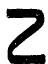
\includegraphics[keepaspectratio]{images/part002_71b18b59.jpg}}

Remarks. 1) In general, the set \(\mathcal{C}(\mathbf{X};\mathbf{Y})\) is not closed in \(\mathcal{F}(\mathbf{X};\mathbf{Y})\) with respect to the topology of pointwise convergence: in other words, a pointwise limit of continuous functions is not necessarily continuous {[}Exercise 5 a){]}.

\begin{enumerate}
\def\labelenumi{\arabic{enumi})}
\setcounter{enumi}{1}
\tightlist
\item
  A filter on \(\mathcal{C}(\mathbf{X};\mathbf{Y})\) can converge pointwise to a continuous function without converging uniformly to this function.
\end{enumerate}

For example, on the interval I = {[}0, 1{]}, let \(u_n\) be the real-valued function which is equal to 0 for \(x = 0\) and \(2/n \leqslant x \leqslant 1\) , equal to 1 for \(x = 1/n\) , and linear in each of the intervals {[}0, 1/n{]} and {[}1/n, 2/n{]}. The sequence \((u_n)\) converges pointwise to 0, but does not converge uniformly to 0 in I (cf.~Exercise 6).

\begin{enumerate}
\def\labelenumi{\arabic{enumi})}
\setcounter{enumi}{2}
\item
  If X is a uniform space, a proof analogous to that of Proposition 8 shows that the set of uniformly continuous mappings of X into Y is closed in \(\mathcal{F}_u(X;Y)\) .
\item
  Suppose that the uniform space Y carries a commutative and associative law of composition, written additively, such that the mapping \((y, y') \to y + y'\) is continuous on \(Y \times Y\) . Then, if \((u_n)\) is a sequence of continuous mappings of X into Y such that the series whose general term is \(u_n\) is uniformly convergent in X, the sum of the series is continuous on X.
\end{enumerate}

We leave it to the reader to state the corresponding result for uniformly summable families (no. 1, Remark 5) of continuous mappings.

PROPOSITION 9. Let X be a topological space, Y a uniform space. Then the mapping \((f, x) \to f(x)\) of \(\mathcal{C}_u(X; Y) \times X\) into Y is continuous.

Let \(f_0: \mathbf{X} \to \mathbf{Y}\) be a continuous mapping, let \(x_0\) be a point of \(\mathbf{X}\) and let \(\mathbf{V}\) be an entourage of \(\mathbf{Y}\) . The set \(\mathbf{T}\) of continuous mappings \(f: \mathbf{X} \to \mathbf{Y}\) such that \((f(x), f(x_0)) \in \mathbf{V}\) for all \(x \in \mathbf{X}\) is a neighbourhood of \(f_0\) in \(\mathcal{C}_u(\mathbf{X}; \mathbf{Y})\) . On the other hand, since \(f_0\) is continuous, there is a neighbourhood \(\mathbf{U}\) of \(x_0\) in \(\mathbf{X}\) such that \((f_0(x), f_0(x_0)) \in \mathbf{V}\) for all \(x \in \mathbf{U}\) . Consequently we have \((f(x), f(x_0)) \in \overset{\circ}{\mathbf{V}}\) whenever \((f, x) \in \mathbf{T} \times \mathbf{U}\) , and the result is proved.

